\chapter{Parallelization}
\label{c:parallelization}

Here we discuss different ways how we can reify the algorithm to support parallelism. There are often several ways of making program parallel. Using parallelization means that there is additionally a need for some communication and synchronization to make the processes arrive at the final result. So it is useful to find as many possible parallelizations, but it is not wise to use all of them.

\section{Process}

The main process of the algorithm as described by dataflow diagram.\cite{Kahn74,Lee95} Circles denote processes and unfinished rectangles denote data stores.

\begin{figure}[H]
	\scalebox{0.8}{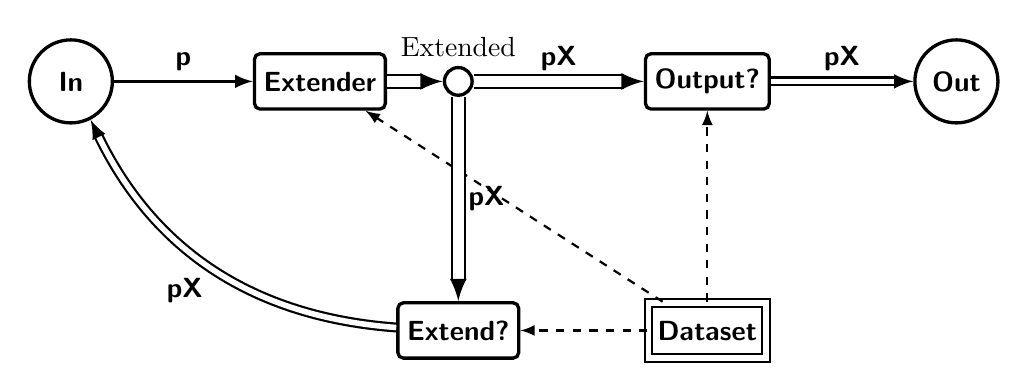
\begin{tikzpicture}[auto]
	\tikzstyle{pool} = [
		draw, very thick, fill=white, 
		circle,
		minimum height=3em, minimum width=3em, 
		node distance=9em, font={\sffamily\bfseries}];
	\tikzstyle{temppool} = [
		draw, very thick, fill=white, 
		circle,
		minimum height=1em, minimum width=1em, 
		node distance=5em, font={\sffamily\bfseries}];

	\tikzstyle{filter} = [
		draw, very thick, fill=white, 
		rectangle, rounded corners=0.2em,
		minimum height=2em, minimum width=4em,
		node distance=9em, font={\sffamily\bfseries}];
	\tikzstyle{extender} = [
		draw, very thick, fill=white, 
		rectangle, rounded corners=0.2em,
		minimum height=2em, minimum width=4em,
		node distance=9em, font={\sffamily\bfseries}];

	\tikzstyle{dataset} = [
		draw, thick, fill=white, 
		rectangle, double, double distance=2pt,
		minimum height=2em, minimum width=4em,
		node distance=9em, font={\sffamily\bfseries}];

	\tikzstyle{take} = [
		very thick, ->, >=latex,
		text centered, font={\sffamily\bfseries}];
	\tikzstyle{chan} = [
		thick, ->, >=latex, double, double distance=4pt,
		text centered, font={\sffamily\bfseries}];
	\tikzstyle{filtered} = [
		thick, ->, >=latex, double, double distance=2pt,
		text centered, font={\sffamily\bfseries}];
	\tikzstyle{needs} = [
		thick, ->, >=latex, dashed,
		text centered, font={\sffamily\bfseries}];

	\node[pool] (in) {In};
	\node[extender, right of=in] (ext) {Extender};
	\node[temppool, right of=ext, label=above:Extended] (exts) {};
	\node[filter, right of=exts] (outable) {Output?};
	\node[filter, below of=exts] (extable) {Extend?};
	\node[pool, right of=outable] (out) {Out};

	\node[dataset, right of=extable] (dataset) {Dataset};
	\draw[needs] (dataset) to (ext);
	\draw[needs] (dataset) to (outable);
	\draw[needs] (dataset) to (extable);

	\draw[take] 
		(in) to node{p} (ext);
	\draw[chan]
		(ext) to (exts);
	\draw[chan] 
		(exts) to node{pX} (outable);
	\draw[chan] 
		(exts) to node{pX} (extable);
	\draw[filtered, bend left] 
		(extable) to node{pX} (in);
	\draw[filtered]
		(outable) to node{pX} (out);
\end{tikzpicture}
}
\end{figure}

We can see that the different query extensions do not share a dependency, except the dataset. Since dataset itself is read-only for a given process, it means we can use multiple extender processes. The same applies for extendability and output filter.

\begin{figure}[H]
  \scalebox{0.8}{\begin{tikzpicture}[auto]
	\node[pool] (in) {In};
	
	% lower part
	\begin{scope}[wrap={label={below:process 2}, inner sep=2ex,fill=black!5}]
		\node[process, below right of=in] (ext1) {Extender};
		\node[process, left of=ext1] (extable1) {Extend?};
		\node[process, right of=ext1] (outable1) {Output?};
	\end{scope}

	\begin{scope}[wrap={label={above:process 1}, inner sep=2ex,fill=black!5}]
		\node[process, above right of=in] (ext2) {Extender};
		\node[process, left of=ext2] (extable2) {Extend?};
		\node[process, right of=ext2] (outable2) {Output?};
	\end{scope}

	\node[dataset, right of=in] (dataset) {Dataset};
	\node[pool, right of=dataset, node distance=12em] (out) {Out};

	\draw[needs] (dataset) to (ext1);
	\draw[needs] (dataset) to (outable1);
	\draw[needs] (dataset) to (extable1);	

	\draw[needs] (dataset) to (ext2);
	\draw[needs] (dataset) to (outable2);
	\draw[needs] (dataset) to (extable2);

	% lower part flow
	\draw[chan, bend left] (in) to node{p} (ext1);
	\draw[chan]	(ext1) to node{pX} (outable1);
	\draw[chan, bend left] (ext1) to node[below]{pX} (extable1);
	\draw[chan, bend left] (extable1) to node[left]{pX} (in);
	\draw[chan, bend right] (outable1) to node[below right]{pX} (out);

	% upper part flow
	\draw[chan, bend right] (in) to node{p} (ext2);
	\draw[chan]	(ext2) to node{pX} (outable2);
	\draw[chan, bend right] (ext2) to node[above]{pX} (extable2);
	\draw[chan, bend right] (extable2) to node[left]{pX} (in);
	\draw[chan, bend left] (outable2) to node{pX} (out);
\end{tikzpicture}
}
\end{figure}

We can add more processes in a similar fashion without affecting the end result. Although such concurrency will introduce a source of indeterminism.

\section{Extending}

The extender can be parallelized via map and reduce concepts\cite{MapReduce,SteeleFold}. The extender was based on two concepts finding the \emph{next} positions from previous pattern position and then group those positions together to find the next queries.

The finding the next position from a position can be easily implemented via mapping by using the \emph{next} function of the dataset. The grouping requires some attention - the grouping is itself a reduction into a map by key with joining.

The pseudo-code representation for such function compositions would be very difficult and would require a lot of new syntax. Therefore we present this idea in Clojure\cite{clojure} which should be readable to people who know lisp. We use the reducers library to show how the extension can be implemented.

\begin{algorithm}[H]
	\caption{Parallel extender}
\begin{lstlisting}[language=Lisp]
(require '[clojure.core.reducers :as r])

; fold-join based grouping function
(defn group-map-by [g f coll]
  (r/fold 
   (r/monoid (partial merge-with into) (constantly {}))
   (fn [ret x]
     (let [k (g x)]
       (assoc ret k (conj (get ret k []) (f x)))))
   coll))

(defn extend [dataset query]
   (let [ steps   (r/mapcat #(walk dataset %) (:positions query))
          grouped (group-map-by :token :position steps)]
        (r/map #(child-query q %) grouped))))
\end{lstlisting}
\end{algorithm}

Such approach may not give much improvement on desktop CPUs, since we already can process multiple queries at the same time. This parallelization could be benefitial for highly parallel processors such as GPGPUs or FPGAs.

\section{Distributed processes}

Since the dataset and the process memory consumption can get quite large it would also be benefitial to be able to partition the dataset between multiple machines. This can also help on a single machine since we can interlace running the different processes and store the non-running process in non-volatile memory.

The extension results for a given query stays inside the sequence which means we can partition by assigning sequences to separate datasets.

The whole dataset is required only for filtering, since even one of the simplest operations ("counting matches in dataset") requires full knowledge of all matches over the dataset. We can calculate partial results and let the filters communicate the results. This could be also done in a seprate process instead of directly communicating.

\begin{figure}[H]
	\scalebox{0.8}{\begin{tikzpicture}[auto]
	\node[pool] (out) {Out};

	% upper part
	\begin{scope}[wrap={label={above:process 1}, inner sep=2ex,fill=black!5}]
		\node[process, above left of=out] (outable1) {Output?};
		\node[process, left of=outable1] (extable1) {Extend?};
		\node[pool,    left of=extable1] (in1) {In};
		\node[process, above of=in1] (ext1) {Extender};

		\node[dataset, above of=outable1] (data1) {Dataset 1};
	\end{scope}

	% lower part
	\begin{scope}[wrap={label={below:process 2}, inner sep=2ex,fill=black!5}]
		\node[process, below left of=out] (outable2) {Output?};
		\node[process, left of=outable2] (extable2) {Extend?};
		\node[pool,    left of=extable2] (in2) {In};
		\node[process, below of=in2] (ext2) {Extender};

		\node[dataset, below of=outable2] (data2) {Dataset 2};
	\end{scope}

	% other
	\draw[needs] (data1) to (ext1);
	\draw[needs] (data1) to (outable1);
	\draw[needs] (data1) to (extable1);

	\draw[needs] (data2) to (ext2);
	\draw[needs] (data2) to (outable2);
	\draw[needs] (data2) to (extable2);

	\draw[chan] (outable1) to (out);
	\draw[chan] (outable2) to (out);

	% upper part flow
	\draw[chan] (in1)  to node{p} (ext1);
	\draw[chan]	(ext1) to node{pX} (extable1);	
	\draw[chan] (extable1) to node{pX} (outable1);
	

	% lower part flow
	\draw[chan] (in2)  to node{p}  (ext2);
	\draw[chan] (ext2) to node{pX} (extable2);
	\draw[chan]	(extable2) to node{pX} (outable2);

	% sync upper
	\draw[sync] (extable1) -- (extable2);
	\draw[sync] (outable1) -- (outable2);
\end{tikzpicture}
}
\end{figure}

\begin{exmp}
For example to see whether some query is over some count limit we first count matches in the partial datasets. Then send the partial results to a each other and add these results together locally. Depending on that result we know how to proceed.
\end{exmp}

Such distribution could be used to separate the process into more managable chunks, but adds significant communication overhead.